\section{Модификация проекта «Интерпретатор арифметических выражений»}
\subsection*{Постановка задачи}
В данном проекте задача была поставлена следующим образом: <<Вычисляются значения выражений, содержащих операцию возведения в степень, обозначаемую символом  \verb|^|, которая считается левоассоциативной и имеет минимальный приоритет>>.

Прежде всего, необходимо учесть, что в отличии от компилятора формул интерпретатор выражнений подразумевает наличие во входной формуле чисел (вместо идентификаторов переменных), а также необходимость выполнения получаемой выходной формулы (результата выражения) вместо её печати. По сути, к действиям, посредством которых был выполнен предыдущий проект, необходимо добавить класс \verb|Calc|, также выведенный из класса \verb|Stack|, и переопределить метод \verb|compile|, который будет вычислять значение входного арифметического выражения после работы соответствующего метода класса \verb|Compf|.

Рассмотрим в качестве входного языка $L(G_0)$ язык правильных арифметических формул, дополненный операцией возведения в степень, являющейся левоассоциативной и имеющей минимальный приоритет. При этом грамматика $G_0$ вышеуказанного языка будет задаваться следующей НФБН:
\\
\begin{center}

\begin{tabular}{rll}
    $F  \rightarrow$ & $T$  &  $| \ F+T \ $  $|$  $ \ F-T $\\
    $T  \rightarrow$ & $M$  &  $| \ T*M \ $  $|$  $ \ T/M $\\
    $M  \rightarrow$ & $F$  &  $| \ M$ \^~$F$ $|$  $ \ V $\\
    $V  \rightarrow$ & $0$  &  $| \ 1  \ | \  2 \  |  ... |  \  9 $\\
\end{tabular} \\
\end{center}
Грамматика $G_S$ выходного языка $L(G_S)$ задаётся такой НФБН: \\

\begin{center}
\begin{tabular}{rll}
	$e  \rightarrow \ e e \ | \ 0 \ | \ 1 \ | \ 2 \ | \ 3 \ | \ ... \ | \ 9 $ \\
\end{tabular}
\end{center}

\subsection*{Теоретические аспекты}
  Класс \verb|Calc| эталонного проекта был создан таким образом, чтобы добавлять новые числа в стек, а при появлении арифметической операции извлекать два числа из стека. Далее, после выполнения требуемого действия результат необходимо класть обратно в стек. При таком подходе, после завершения компиляции формулы, на вершине стекового калькулятора окажется результат вычисления арифметического выражения.
\subsection*{Описание используемых структур и применяемых алгоритмов}
 В данном случае суть модификации состояла в добавлении нового метода \\ \verb|involution|, определяющего операцию. Так как дополнительными условиями данной задачи являются минимальный приоритет и левоассоциативность операции, необходимо для правильной обработки случая, когда нам встречается данная операция, переопределить метод \verb|process_oper|:


\begin{lstlisting}

def involution(a,n)
  result =1
  if n>1
    n.times do
      result*=a
    end
  elsif n==1
    result=a
  elsif n==0
    result=1
  end
  return result
end

def process_oper(c)
    if c =='^'
      second,first = @s.pop,@s.pop
      @s.push(involution(first,second))
    else
    second, first = @s.pop, @s.pop
    @s.push(first.method(c).call(second))
    end
end
\end{lstlisting}

Ниже проиллюстрирован результат работы программы:
\begin{figure}[ht!]
\begin{center}
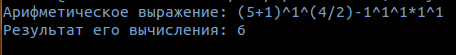
\includegraphics[width=0.8\hsize]{images/screen2}
\end{center}
\caption{Вывод программы}\label{fig:screen2}
\end{figure}
